\documentclass[10pt,a4paper]{article}

% ── Packages ──────────────────────────────────────────────────────────────────
\usepackage[T1]{fontenc}
\usepackage[utf8]{inputenc}

% Font Configuration: Scale Helvetica and Courier for a balanced, modern look
\usepackage[scaled=0.92]{helvet}
\usepackage[scaled=0.95]{courier}
\renewcommand{\familydefault}{\sfdefault}

% Adjusted geometry to leave proper header and footer margins, preventing overlaps
\usepackage[margin=1.8cm, top=2.2cm, bottom=2.2cm, headheight=15pt, headsep=10pt, footskip=12pt]{geometry}
\usepackage{microtype}
\usepackage{booktabs}
\usepackage{tabularx}
\usepackage{array}
\usepackage{multirow}
\usepackage{enumitem}
\usepackage{titlesec}
\usepackage{fancyhdr}
\usepackage{setspace} % For professional line spacing adjustments
\usepackage{needspace}
\usepackage{parskip} % Modern paragraph spacing (no indent, clean vertical gaps)
\raggedbottom

\usepackage{mdframed}
\usepackage{verbatim}
\usepackage{listings}
\usepackage{amsmath}
\usepackage{hyperref}
\usepackage{xcolor}  % required by listings but palette restricted to black/white
\usepackage{graphicx}
\usepackage{tikz}
\usetikzlibrary{shapes.geometric, arrows.meta, positioning, calc}
\usepackage{float}
\usepackage{caption}

% Set line spacing to 1.15 for better readability and a professional feel
\setstretch{1.15}

% ── Black-and-white only ──────────────────────────────────────────────────────
\hypersetup{colorlinks=false, pdfborder={0 0 0}}

% ── Typography ────────────────────────────────────────────────────────────────
\lstset{
  basicstyle=\ttfamily\small,
  breaklines=true,
  frame=single,
  framerule=0.6pt,
  rulecolor=\color{black!80},
  backgroundcolor=\color{black!3},
  xleftmargin=8pt,
  xrightmargin=8pt,
  aboveskip=8pt,
  belowskip=8pt,
}

% ── Section formatting (Modern, clean ruled lines) ────────────────────────────
\titleformat{\section}[block]
  {\normalfont\large\bfseries}
  {}
  {0pt}
  {}
  [\vspace{2pt}\titlerule]

\titleformat{\subsection}[block]
  {\normalfont\normalsize\bfseries}
  {}
  {0pt}
  {}

\titlespacing*{\section}{0pt}{14pt}{6pt}
\titlespacing*{\subsection}{0pt}{10pt}{4pt}

% ── List settings ─────────────────────────────────────────────────────────────
\setlist[itemize]{topsep=4pt, itemsep=3pt, parsep=0pt, leftmargin=15pt}
\setlist[enumerate]{topsep=4pt, itemsep=3pt, parsep=0pt, leftmargin=15pt}

% ── Table settings ────────────────────────────────────────────────────────────
\renewcommand{\arraystretch}{1.3} % Add padding to tables for professional aesthetics

% ── Header / footer ───────────────────────────────────────────────────────────
\pagestyle{fancy}
\fancyhf{}
\renewcommand{\headrulewidth}{0pt}
\fancyfoot[C]{\footnotesize\thepage}

% ── Table of Contents Styling (Clean, Professional hierarchy) ─────────────────
\usepackage[titles]{tocloft}
\setcounter{secnumdepth}{0} % Remove automatic section numbering since manual Roman numerals are used

% Style Section entries (indented under Parts, with dot leaders)
\renewcommand{\cftsecleader}{\cftdotfill{\cftdotsep}}
\cftsetindents{section}{1.5em}{2.5em}
\setlength{\cftbeforesecskip}{4pt}

% Style Part entries (unindented, bold, with extra spacing)
\setlength{\cftbeforepartskip}{12pt}
\renewcommand{\cftpartfont}{\normalfont\normalsize\bfseries}
\renewcommand{\cftpartpagefont}{\normalfont\normalsize\bfseries}
\renewcommand{\cftpartleader}{\cftdotfill{\cftdotsep}}

% ── Tight rule box (with light grey background, professional border) ──────────
\newmdenv[
  linewidth=0.8pt,
  linecolor=black!70,
  backgroundcolor=black!3,
  innerleftmargin=10pt,
  innerrightmargin=10pt,
  innertopmargin=8pt,
  innerbottommargin=8pt,
  skipabove=10pt,
  skipbelow=10pt,
  roundcorner=3pt,
  nobreak=true
]{rulebox}

% ── Prevent Widows and Orphans ────────────────────────────────────────────────
\clubpenalty=10000
\widowpenalty=10000
\displaywidowpenalty=10000

% ──────────────────────────────────────────────────────────────────────────────
\begin{document}
% ──────────────────────────────────────────────────────────────────────────────

% ── TITLE BLOCK ───────────────────────────────────────────────────────────────
\begin{center}
{\LARGE\bfseries BOI Hackathon 2026}\\[4pt]
{\large Unified AI Solutions for Cybersecurity \& Financial Intelligence}\\[8pt]
\rule{\linewidth}{1.2pt}\\[6pt]
\begin{tabularx}{\linewidth}{lX}
\textbf{Team:} & Hunters \\
\textbf{Members:} & Galipalli Pranav Raj (Lead), Abhinav Mucharla, Pranav Krishna, Siri Chandana \\
\textbf{Submission Category:} & Problem Statement 1 (Primary) \\
\textbf{Solution Title:} & Kavach.ai (PS1)
\end{tabularx}\\[4pt]
\rule{\linewidth}{0.6pt}
\end{center}

\vspace{6pt}

% ── Table of Contents ──────────────────────────────────────────────────────────
\tableofcontents
\newpage

% ══════════════════════════════════════════════════════════════════════════════
\section*{PART ONE: PRIMARY FOCUS (PROBLEM STATEMENT 1)}
\addcontentsline{toc}{part}{PART ONE: PRIMARY FOCUS (PROBLEM STATEMENT 1)}
% ══════════════════════════════════════════════════════════════════════════════

% ══════════════════════════════════════════════════════════════════════════════
\section{I. EXECUTIVE SUMMARY}
% ══════════════════════════════════════════════════════════════════════════════

The Indian mobile banking ecosystem faces an accelerating crisis. Financially motivated threat actors deploy mutated Android applications that bypass traditional signature-based defenses, intercept OTPs, hijack UPI sessions, and drain accounts before any human analyst can respond. Security Operations Centers relying on \textbf{manual reverse engineering} introduce a critical \textbf{defense lag} that modern banking trojans are specifically engineered to exploit.

\textbf{Kavach.ai} is a \textbf{fully automated, dual-track forensic pipeline} that eliminates this lag. It accepts an untrusted APK, subjects it to \textbf{simultaneous static code analysis and live behavioral sandbox observation}, fuses both intelligence streams through a schema-enforced reasoning engine, and produces a calibrated risk score, a MITRE ATT\&CK mapped threat report, and a pre-filled CERT-In compliance submission, all within a \textbf{sub-30-second processing target} (delivering preliminary triage and structured reports in under 30 seconds, with complete dynamic sandbox confirmation completing asynchronously).

The pipeline's core innovation is its layered approach to automated security analysis: producing reliable, auditable conclusions without human oversight. Kavach.ai achieves this through three key pillars. First, a \textbf{cybersecurity-native transformer} (SecureBERT-2.0) trained on mathematically extracted behavioral chains, making it resilient to code obfuscation. Second, a \textbf{live behavioral observation layer} (local MobSF + Objection + eBPF dynamic sandbox) that executes the APK and collects user-land and kernel-land logs. Third, a \textbf{structured hallucination prevention framework} (Pydantic schema constraints) that forces the reasoning engine (LLaMA-3) to only report what the evidence proves, never what it imagines.

The result is a system designed to produce forensic output that a SOC analyst, a compliance auditor, and a regulatory body can all \textbf{independently verify}.

% ══════════════════════════════════════════════════════════════════════════════
\section{II. THE THREAT LANDSCAPE \& USE CASES}
% ══════════════════════════════════════════════════════════════════════════════

\subsubsection*{The Active Indian Banking Trojan Ecosystem}

The threat landscape Kavach.ai is designed to address is not generic mobile malware. It is a specific, well-documented family of financially motivated Android trojans targeting Indian payment infrastructure. Understanding their specific attack mechanisms is essential to understanding every architectural decision in the pipeline.

\textbf{Dynamic Droppers (e.g. NexusRoute campaigns):} These threats distribute malicious APKs containing minimal static signatures, relying on dynamic class loading (\texttt{DexClassLoader}) to download and execute secondary payloads from C2 servers at runtime. They often use the Java Native Interface (JNI) to hide core logic inside compiled native libraries (\texttt{.so} files) and deploy explicit anti-analysis checks (such as emulator and build-profile inspection) to evade standard sandboxes.

\textbf{Credential \& SMS Interceptors (e.g. EventBot, Drinik, ToxicPanda):} These trojans exploit Android's Accessibility Services framework to harvest active credentials and overlay fake login interfaces over legitimate banking applications. They also acquire SMS-reading privileges (\texttt{READ\_SMS} and \texttt{RECEIVE\_SMS}) to intercept and extract OTPs, enabling autonomous unauthorized transfers before the victim receives any notification.

These trojans share three architectural properties that define the requirements for any effective detection system. They use obfuscation to defeat static signature matching. They use anti-analysis evasion to defeat dynamic sandbox observation. And they use the gap between static and dynamic findings (appearing clean in one context while being malicious in another) as a deliberate evasion technique. Kavach.ai is designed specifically around closing all three gaps simultaneously.

\subsubsection*{Use Cases}

\begin{itemize}
  \item \textbf{SOC Automated Triage:} Reduces forensic analysis time from hours to under 30 seconds per sample, automatically prioritizing the queue by risk severity and producing analyst-ready reports.
  \item \textbf{Regulatory Compliance Automation:} Automatically maps forensic output to the official CERT-In Incident Reporting Form, enabling immediate compliance within the mandatory 6-hour reporting window.
  \item \textbf{RBI DPSC Alignment:} Automatically flags ProGuard/DexGuard indicators, overlay vulnerabilities (\texttt{SYSTEM\_ALERT\_WINDOW}), and non-genuine application tampering to meet RBI's Master Direction.
\end{itemize}

% ══════════════════════════════════════════════════════════════════════════════
\section{III. CORE ARCHITECTURE: THE 7-STAGE FORENSIC PIPELINE}
% ══════════════════════════════════════════════════════════════════════════════

\subsubsection*{Architectural Overview}

\begin{figure}[H]
  \centering
  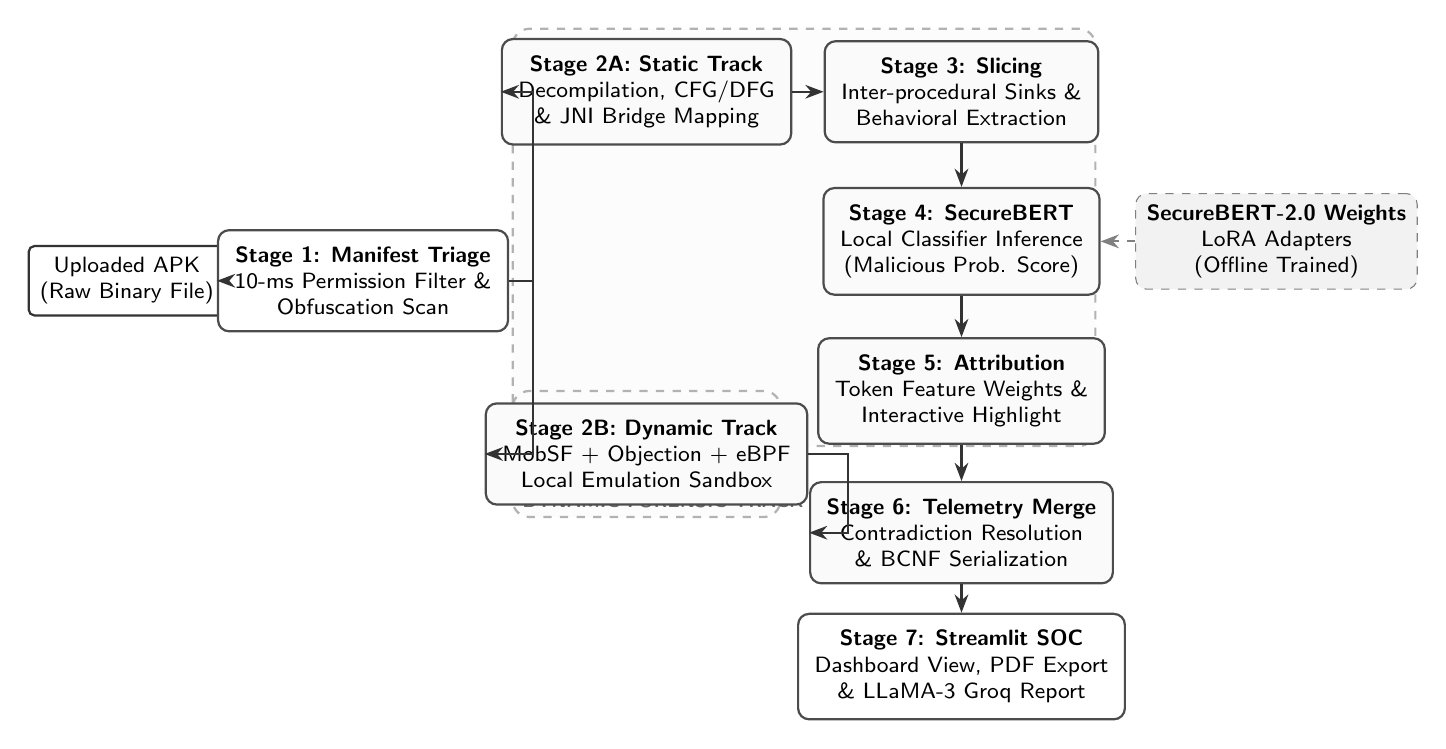
\begin{tikzpicture}[
    node distance=1.5cm and 1.2cm,
    font=\sffamily\footnotesize,
    >=Stealth,
    % Styles
    card/.style={
      draw=black!70,
      fill=black!2,
      thick,
      rounded corners=4pt,
      align=center,
      minimum width=3.0cm,
      minimum height=1.1cm,
      inner sep=6pt
    },
    inputcard/.style={
      draw=black!80,
      fill=white,
      thick,
      rounded corners=2pt,
      align=center,
      minimum width=2.2cm,
      minimum height=0.8cm,
      inner sep=4pt
    },
    modelcard/.style={
      draw=black!50,
      fill=black!5,
      dashed,
      rounded corners=4pt,
      align=center,
      minimum width=2.8cm,
      minimum height=1.0cm,
      inner sep=4pt
    },
    groupbox/.style={
      draw=black!30,
      dashed,
      thick,
      rounded corners=6pt,
      fill=black!1
    },
    grouplabel/.style={
      font=\sffamily\scriptsize\bfseries,
      text=black!60
    },
    arrow/.style={
      ->,
      thick,
      draw=black!80
    },
    dashedarrow/.style={
      ->,
      thick,
      dashed,
      draw=black!50
    }
  ]

    % Group boxes drawn first so they are naturally in the background
    \draw [groupbox] (1.1, 3.2) rectangle (8.5, -2.1);
    \draw [groupbox] (1.1, -1.4) rectangle (4.5, -3.0);

    % Group Labels
    \node[anchor=north west, grouplabel] at (1.1, 3.2) {STATIC FORENSIC TRACK};
    \node[anchor=south west, grouplabel] at (1.1, -3.0) {DYNAMIC FORENSIC TRACK};

    % Coordinates and Nodes
    \node (apk) [inputcard] at (-3.8, 0) {Uploaded APK\\(Raw Binary File)};
    \node (s1) [card, fill=white] at (-0.8, 0) {\textbf{Stage 1: Manifest Triage}\\10-ms Permission Filter \&\\Obfuscation Scan};

    % Static Track Nodes
    \node (s2a) [card] at (2.8, 2.4) {\textbf{Stage 2A: Static Track}\\Decompilation, CFG/DFG\\\& JNI Bridge Mapping};
    \node (s3) [card] at (6.8, 2.4) {\textbf{Stage 3: Slicing}\\Inter-procedural Sinks \&\\Behavioral Extraction};
    \node (s4) [card] at (6.8, 0.5) {\textbf{Stage 4: SecureBERT}\\Local Classifier Inference\\(Malicious Prob. Score)};
    \node (s5) [card] at (6.8, -1.4) {\textbf{Stage 5: Attribution}\\Token Feature Weights \&\\Interactive Highlight};

    % Model Weights
    \node (weights) [modelcard] at (10.8, 0.5) {\textbf{SecureBERT-2.0 Weights}\\LoRA Adapters\\(Offline Trained)};

    % Dynamic Track Node
    \node (s2b) [card] at (2.8, -2.2) {\textbf{Stage 2B: Dynamic Track}\\MobSF + Objection + eBPF\\Local Emulation Sandbox};

    % Merge and Output Nodes
    \node (s6) [card] at (6.8, -3.2) {\textbf{Stage 6: Telemetry Merge}\\Contradiction Resolution\\\& BCNF Serialization};
    \node (s7) [card, fill=white] at (6.8, -4.9) {\textbf{Stage 7: Streamlit SOC}\\Dashboard View, PDF Export\\\& LLaMA-3 Groq Report};

    % Connections
    \draw [arrow] (apk) -- (s1);
    
    % Split from S1 to S2a and S2b
    \draw [arrow] (s1.east) -- ++(0.3,0) |- (s2a.west);
    \draw [arrow] (s1.east) -- ++(0.3,0) |- (s2b.west);

    % Static Track Flow
    \draw [arrow] (s2a) -- (s3);
    \draw [arrow] (s3) -- (s4);
    \draw [arrow] (s4) -- (s5);
    \draw [dashedarrow] (weights) -- (s4);

    % Dynamic Track Flow
    \draw [arrow] (s2b.east) -- ++(0.5,0) |- (s6.west);

    % Merge and Final Output Flow
    \draw [arrow] (s5) -- (s6);
    \draw [arrow] (s6) -- (s7);

  \end{tikzpicture}
  \caption{Kavach.ai APK Forensic Pipeline Core Architecture}
  \label{fig:pipeline_ps1}
\end{figure}

\subsubsection*{Stage 1: Manifest Triage and 10-Millisecond Triage Filter}

This stage operates as the first line of defense. Utilizing Androguard, the pipeline unzips the APK and extracts the raw \texttt{AndroidManifest.xml} in under 10 milliseconds, parsing permission declarations and entry points. The triage engine evaluates permission combinations rather than individual permissions in isolation, flagging malicious indicators like accessibility service abuse (\texttt{BIND\_ACCESSIBILITY\_SERVICE} with \texttt{RECEIVE\_SMS} and \texttt{SYSTEM\_ALERT\_WINDOW}) or persistence-focused droppers (\texttt{REQUEST\_INSTALL\_PACKAGES} with \texttt{RECEIVE\_BOOT\_COMPLETED}) to instantly prioritize high-risk files.

To prevent evasion via dynamic class loading and java reflection, this stage incorporates a \textbf{Reflection \& Obfuscation Density Scan}. If Androguard detects a disproportionately high density of reflection indicators (such as \texttt{Class.forName}, \texttt{getMethod}, or \texttt{invoke}) paired with high-entropy cryptographic byte-arrays and low readable text content, it flags the app as an anomalous threat. This bypasses the subsequent static decompilation slicing phase and routes the APK directly to the heavy dynamic sandbox with an elevated prior risk rating.

Because advanced malware may declare minimal permissions and acquire capabilities dynamically, this stage never issues a final verdict or terminates the pipeline. Instead, it generates a triage priority score that determines the submission's position in the deep analysis queue. This ensures that high-signal samples are prioritized immediately under operational Security Operations Center workloads. Crucially, the permission combination flags generated in this stage are carried forward as metadata to Stage 6, serving as corroborating prior evidence that directly feeds into the final report's risk profiling.

\subsubsection*{Stage 2A: Static Track: Decompilation, Graph Construction, and Native Binary Triage}

The static track reverse-engineers the APK binary using APKTool to extract Smali bytecode, with parallel JADX decompilation for fallback analysis. To ensure resilience against obfuscation strategies designed to crash compiler abstract syntax trees (ASTs)—such as intentionally malformed ZIP headers or invalid character injections—the parser implements a \textbf{Smali Fallback} mechanism. If standard decompiler translation fails, the system bypasses AST generation and falls back directly to raw Smali text extraction, preserving the Dalvik opcodes to ensure backward program slicing remains fully operational.

Kavach.ai eliminates native-code blindspots by auditing binary native libraries (\texttt{.so} files) in the APK's \texttt{/lib} directory. The static track runs a sub-process executing an ELF parser or raw byte-scanner on the compiled C/C++ binaries. By actively mapping dynamic JNI exports using the standard \texttt{Java\_package\_class\_method} naming convention, the pipeline establishes a \textbf{JNI Bridge} that maps relations between the Java bytecode layer and compiled C/C++ native entry points. If a native library references low-level system call hooks (like direct socket bindings, reverse-shell execution, or direct memory scraping), the scanner flags the native library as a critical threat vector and instructs the dynamic sandbox to explicitly monitor these runtime triggers.

Androguard then processes the bytecode to construct a Control Flow Graph (mapping execution paths) and a Data Flow Graph (tracking value transformations). Together, these graphs provide the formal mathematical representation of program execution that the backward slicing algorithm traverses.

\subsubsection*{Stage 2B: Dynamic Track: Local "Holy Trinity" Sandbox (MobSF + Objection + eBPF)}

Simultaneously, the APK is routed to our local dynamic analysis pipeline, combining \textbf{MobSF}, \textbf{Objection}, and \textbf{eBPF} to observe malware behavior at both user-land and kernel-land. This local stack completely eliminates the dependencies, privacy concerns, and latency of cloud-based APIs like Any.run.

The execution is automated and orchestrated in under 20 seconds:
\begin{itemize}
  \item \textbf{Environment Setup (MobSF):} MobSF manages the local emulation workspace, boots the root-enabled ARM64 Android emulator, installs the target APK, and runs the local Frida server on the emulator.
  \item \textbf{User-Land Breach (Objection):} To strip away surface-level defenses, the orchestrator executes an \texttt{objection} subprocess to hook the app process and bypass root checks and SSL pinning, forcing the malware to expose its decrypted network and payload traffic:
  \begin{lstlisting}[language=bash]
objection -g <package_name> explore -s "android root disable" -s "android sslpinning disable"
  \end{lstlisting}
  \item \textbf{Kernel-Land Stealth Observation (eBPF):} To counter anti-Frida and anti-analysis evasion tactics where modern banking trojans self-destruct upon detecting user-land instrumentation, the orchestrator uses ADB to push a pre-compiled eBPF tracing probe directly into the emulator's Linux kernel before app launch. The probe monitors raw system calls (syscalls), file descriptors, and socket connections completely invisible to the user-land process.
  \item \textbf{Detonation \& Collection:} The orchestrator broadcasts system intents (such as \texttt{BOOT\_COMPLETED} or \texttt{BATTERY\_LOW}) via ADB to wake up dormant malware components. Objection dumps decrypted memory spaces while the eBPF probe captures stealthy kernel-level logs, merging both outputs into a unified JSON file for analysis.
\end{itemize}

To override delayed execution loops (such as \texttt{Thread.sleep}), the pipeline uses Frida script hooks to intercept dynamic runtime delay APIs (such as \texttt{SystemClock.sleep} or \texttt{Handler.postDelayed}) and fast-forwards the clock tickers. To resolve null pointer exceptions when injecting Frida hooks into native code, the interceptor hooks the \texttt{System.loadLibrary} or \texttt{dlopen} calls, delaying memory attachment until the library is fully resident in RAM.

This local pipeline runs entirely within our secure, air-gapped system, ensuring sensitive financial samples never leave the organization.

\subsubsection*{Stage 3: Backward Program Slicing: From Codebase to Behavioral Chain}

To align the codebase with SecureBERT-2.0's 1024-token limit, Kavach.ai implements inter-procedural backward program slicing based on the LAMD framework (Feb 2025). The algorithm flags suspicious API sinks (e.g. \texttt{SmsManager.sendTextMessage}, \texttt{DexClassLoader.loadClass}, \texttt{MediaProjection} calls, or \texttt{AccessibilityService.onEvent}) and performs a backward traversal of the Control and Data Flow Graphs.

This traversal traces dependencies across function boundaries, discarding unrelated code and extracting only the precise instruction sequences that feed into the dangerous sinks. Native library (\texttt{.so}) boundaries are resolved via static string extraction to recover C2 addresses and hardcoded payloads, appending them to the static findings. To handle encrypted or obfuscated native code blocks, the slicing engine computes a \textbf{Native Opacity Score} based on high-entropy native segments and unresolved JNI calls; if JNI boundaries are hit without readable static payloads, this opacity metric is passed forward to Stage 6 to prevent silent analysis evasion.

\subsubsection*{Stage 4: SecureBERT-2.0 Deep Semantic Classification}

The extracted slices are tokenized and processed by SecureBERT-2.0 (our custom-trained domain-specific transformer based on the ModernBERT backbone [6], pre-trained on 13.6B cybersecurity tokens and 53.3M code tokens). Pretraining gives the model a native semantic understanding of malicious chains that general-purpose models (e.g. CodeBERT) lack.

SecureBERT-2.0 outputs a malicious probability score between 0.0 and 1.0. Because multiple slices may be extracted per APK, the final score is the maximum of all slice scores. To minimize single-slice false positives (e.g. from legitimate screen readers or assistive tools utilizing accessibility APIs), the aggregation engine supports dual-mode decision thresholds: either a single slice score exceeding a high-confidence threshold ($\geq 0.85$), or two or more independent slices concurrently scoring above a lower threshold ($\geq 0.60$), allowing the bank to tune the precision/recall trade-off based on its operational risk appetite. As an encoder-only classification model, it cannot fabricate evidence or hallucinate, outputting a deterministic probability score.

\subsubsection*{Stage 5: SHAP Feature Attribution, Latency Mitigation, and Interactive Highlighting}

A probability score of 0.87 is not a forensic finding. A security analyst cannot take a number to a compliance audit. A court cannot evaluate a number as evidence. The SHAP attribution layer transforms the model's numerical output into a specific, token-level account of which elements of the code drove the classification decision.

SHAP, Shapley Additive Explanations, calculates the marginal contribution of each input token to the model's output score by systematically evaluating how the score changes when each token is present versus absent. To maintain a sub-second latency budget on execution, Kavach.ai avoids brute-force KernelSHAP on full sequences, implementing \textbf{PartitionSHAP} or \textbf{FastSHAP} which leverage hierarchical clustering trees to evaluate token groups. The system also performs \textbf{targeted truncation}, strictly capping inputs to the top 3 critical code blocks from Androguard's traversal, ensuring explainability computations finish in under 1.5 seconds.

For a given code slice, this produces a ranked list of tokens with associated weights:
\begin{rulebox}
\begin{verbatim}
getContacts()                +0.38   strongly pushed toward malicious
sendTextMessage()            +0.29   strongly pushed toward malicious
Base64.encode()              +0.21   pushed toward malicious
"+19876543210"               +0.18   pushed toward malicious (hardcoded number)
setContentView()             -0.04   slightly pushed toward benign
\end{verbatim}
\end{rulebox}

This attribution serves three functions in the pipeline. First, it provides the specific evidence excerpts that the merge layer passes to LLaMA-3, grounding the generative report in concrete code-level observations rather than model-level abstractions. Second, it creates an independently verifiable audit trail. A human analyst can look at the flagged tokens, examine the corresponding lines in the decompiled code, and confirm that the model's reasoning is grounded in real behavior. Third, it provides the feature-level explanation that satisfies regulatory requirements for auditable automated decision systems.

Furthermore, to visualize these explanations interactively, the Streamlit dashboard features a custom **SHAP Highlight Renderer**. This interface physically renders the Smali bytecode on the screen: tokens that push the classification towards "Malicious" are illuminated with a red glow, while "Benign" tokens glow blue. This provides analysts with an intuitive, visual proof of the model's decision boundaries.

The SHAP explainer is fitted once during the offline training phase on the validation partition and frozen before deployment. This ensures that attribution calculations during inference reflect the same model state that was evaluated during training.

\subsubsection*{Stage 6: Cross-Layer Telemetry Merge, Database Serialization, and Graceful Degradation}

This stage fuses numerical probabilities, static permission metadata carried forward from Stage 1, and dynamic sandbox observations into a structured report using a three-layer validation system, subsequently serializing findings to a normalized PostgreSQL database backend to ensure transactional data integrity.

\paragraph{Layer 1: Input Schema Enforcement \& Database Serialization}
Validates static findings (probability score, SHAP tokens, code slice) and dynamic observations (IP addresses, SMS activity, API calls) against strict Pydantic schemas. The orchestrator maps and writes these validated metrics into a normalized PostgreSQL relational model structured up to BCNF (incorporating dedicated tables for \texttt{apks}, \texttt{smali\_slices}, \texttt{shap\_attributions}, and \texttt{cert\_in\_reports}), safeguarding data records against modification anomalies.

\paragraph{Layer 1.5: Post-Detonation Local State Scraping}
To defeat dynamic payload encryption and obfuscated dynamic channels, the pipeline implements post-detonation local state filesystem scraping. Upon completion of sandbox execution, the orchestrator programmatically scrapes the sandbox filesystem directory \texttt{/data/user/0/<package\_name>}. It extracts cleartext XML Shared Preferences files, dynamically decrypted SQLite databases, and local session caches containing cleartext command-and-control (C2) domains and dynamic encryption keys, passing these artifacts directly to the merge layer to bypass network-level inspection limitations.

\paragraph{Layer 2: Deterministic Contradiction Resolution}
Compares static and dynamic findings using explicit logical rules, assigning a contradiction flag to override LLM behavior:
\begin{itemize}
  \item \textbf{\texttt{CONFIRMED\_MALWARE} (Both tracks high):} Fuses tracks and reports at combined severity level.
  \item \textbf{\texttt{PACKED\_DROPPER} (Static low, Dynamic high):} Identifies dynamic runtime loader activity; overrides risk score floor to 85.
  \item \textbf{\texttt{DORMANT\_MALWARE} (Static high, Dynamic low):} Identifies potential sandbox evasion; retains HIGH rating based on static evidence.
  \item \textbf{\texttt{SANDBOX\_EVASION\_DETECTED} (Static low/medium, Dynamic evasion high):} Triggered when local eBPF kernel tracing or Objection hooks report anti-VM/anti-emulator indicators or abnormal early process exits; overrides final score to a minimum of 75.
  \item \textbf{\texttt{LIKELY\_BENIGN} (Both tracks low):} Flags application as low risk and caps final score at 30.
\end{itemize}

\paragraph{Layer 3: Output Schema Enforcement \& Graceful Degradation}
Validates LLaMA-3 outputs against a Pydantic schema requiring structured MITRE ATT\&CK identifiers and direct token-level citations to SHAP or dynamic logs. For example, if the static analysis flags an Accessibility Service exploitation sink, the output schema enforces a mapping to \textbf{MITRE ATT\&CK Technique T1417 (Input Capture)} with direct code citations, grounding the threat label in concrete code behavior. The LLM acts purely as a structured compiler, preventing AI hallucinations.

To prevent the Streamlit UI from throwing runtime exceptions if a chaotic malware string causes formatting slips or schema failures, the Groq parser incorporates a **Graceful Degradation** mechanism. The Pydantic validator is wrapped in try/except blocks; if strict validation fails, the engine falls back to a **Regex Recovery Parser** that extracts critical fields (such as threat classification, final score, and MITRE codes) from the raw LLM output, failing over to a clean pre-formatted markdown template so that the dashboard remains operational.

\needspace{10\baselineskip}
\subsubsection*{Final Risk Score Calculation}
\begin{rulebox}
\begin{verbatim}
base_score = securebert_probability * 100

dynamic_modifiers:
  confirmed C2 network connection:   +10 points
  SMS exfiltration observed:         +15 points
  banking database accessed:         +10 points
  root escalation attempted:         +12 points
  DexClassLoader at runtime:         +8 points

contradiction_overrides:
  PACKED_DROPPER flag:          floor(score, 85)
  DORMANT_MALWARE flag:         retain static score, no dynamic discount
  SANDBOX_EVASION_DETECTED flag: floor(score, 75)
  CONFIRMED_MALWARE flag:       apply all dynamic modifiers
  LIKELY_BENIGN flag:           cap score at 30 unless static exceeds 0.5

final_score_pre_override = min(base_score + dynamic_modifiers, 100)
final_score = apply_contradiction_overrides(final_score_pre_override)

severity_mapping:
  80-100:  CRITICAL
  60-79:   HIGH
  40-59:   MEDIUM
  0-39:    LOW
\end{verbatim}
\end{rulebox}

Contradiction overrides are applied to the final score as a post-processing step after the base score and dynamic modifiers are summed.

\subsubsection*{Decoupled Microservices, Latency Budget, and Asynchronous Orchestration}

To avoid the monolithic bottleneck where heavy static calculations and dynamic sandboxing block the user interface, Kavach.ai separates execution into a decoupled microservices architecture utilizing a Streamlit frontend, a FastAPI asynchronous orchestrator, and a normalized PostgreSQL state manager.

Under the FastAPI asynchronous model ("Restaurant Ticket" paradigm), the API accepts incoming APK binaries, vaults them in the local PostgreSQL database (stashed as secure BYTEA payloads or local secure offline storage), records an execution transaction in PostgreSQL, and immediately hands a unique \texttt{Job ID} ticket back to the Streamlit client. The heavy analysis is then routed to background Celery or ARQ worker processes, freeing the API to process concurrent requests.

The Streamlit dashboard implements client-side polling, sending light requests to the FastAPI backend every two seconds using the \texttt{Job ID} ticket:
\begin{itemize}
  \item While the database status registers as \texttt{Analyzing}, the UI displays a loading spinner.
  \item When the database status updates to \texttt{Completed}, the UI retrieves the structured threat payload and renders the dashboard.
\end{itemize}

This asynchronous orchestration balances SOC concurrency requirements and fits a strict operational timeline:
\begin{itemize}
  \item \textbf{Synchronous Forensic Track (10--15 Seconds):} Runs the triage filter (~10\,ms), Smali extraction and backward slicing (~5.0\,s), SecureBERT-2.0 inference (~0.8\,s), SHAP token attribution (~1.5\,s), and LLaMA-3 report compilation via Groq API (~1.2\,s). This yields a complete, auditable report and preliminary risk score in under 15 seconds.
  \item \textbf{Asynchronous Dynamic Track (15--20 Seconds):} Runs in parallel. The orchestrator calls the local MobSF service to boot the emulator, injects root-bypass and SSL-pinning hooks via Objection, and inserts the stealthy eBPF kernel probe. Telemetry is gathered for a 15-second observation window and returned immediately.
  \item \textbf{Dynamic Dashboard Update:} Once the dynamic track finishes, the Streamlit dashboard updates the score and merges the user-land memory dumps and kernel-space logs into the active case file without requiring any manual analyst refresh.
\end{itemize}

\subsubsection*{Stage 7: Operational Deployment: Streamlit SOC Dashboard}
The entire multi-stage pipeline is exposed via a Python-native \textbf{Streamlit} dashboard, serving as the central operational hub for SOC analysts. Rather than interacting with abstract scripts, analysts use the dashboard for drag-and-drop binary uploads (APKs), real-time execution tracking, and interactive visualizations of the SHAP feature attributions. The interface renders the final LLaMA-3 case files dynamically, allowing for one-click PDF exports of the CERT-In compliance reports, shifting Kavach.ai from a backend engine into a fully deployable software asset.

% ══════════════════════════════════════════════════════════════════════════════
\section{IV. DIFFERENTIATION \& STRATEGIC ADVANTAGE}
% ══════════════════════════════════════════════════════════════════════════════

\begin{tabularx}{\linewidth}{>{\bfseries}p{0.22\linewidth}X}
\toprule
Advantage & Technical Basis \\
\midrule
Obfuscation Resistance & Extracts inter-procedural data-flow relationships instead of cosmetic method names. The extracted behavioral chain remains structurally identical under code obfuscation and renaming. \\
\addlinespace
Runtime Payload Detection & Captures execution events of runtime droppers (e.g. NexusRoute) that dynamically load code in memory via \texttt{DexClassLoader}, bypassing all static inspection. \\
\addlinespace
Contradiction Logic & Treats track conflicts as primary indicators: statically clean but dynamically active signals a \texttt{PACKED\_DROPPER} (score floored at 85); statically suspicious but dynamically silent suggests a sandbox-evading \texttt{DORMANT\_MALWARE}. \\
\addlinespace
Zero-Hallucination GenAI & Constrains LLaMA-3 through Pydantic input/output schemas and deterministic rules. The LLM acts purely as a structured reporting compiler, completely preventing generated fabrications. \\
\addlinespace
Hourly Threat Sync & Continuously ingests fresh banking trojan feeds from MalwareBazaar into LoRA adapters, updating analysis seeds and detection weights within hours without full model retraining. \\
\bottomrule
\end{tabularx}

\subsection*{Architectural Concurrency Pitch}

We engineered Kavach.ai for enterprise concurrency. We decoupled the presentation layer from the execution layer using an asynchronous FastAPI orchestrator. Malware artifacts are isolated in an S3-compatible vault, while a normalized PostgreSQL database tracks the state machine of the SOC pipeline. This ensures our AI can process massive queues of financial threats in the background without ever bottlenecking the human analyst's dashboard.

% ══════════════════════════════════════════════════════════════════════════════
\section{V. DATA ENGINEERING \& TECHNOLOGY STACK}
% ══════════════════════════════════════════════════════════════════════════════

\subsubsection*{Training Corpora and Diversity Metrics}

The offline fine-tuning phase relies on a multi-source dataset matrix covering over a decade of malware evolution across hundreds of distinct behavioral families and obfuscation techniques:
\begin{itemize}
  \item \textbf{AMD (Argus Lab) [9] (24,650 samples):} The primary behavioral ground truth corpus. Documents 71 distinct malware families across 135 behavioral varieties collected between 2010 and 2016. Its detailed behavioral taxonomy acts as the semantic anchor for SecureBERT-2.0's fine-tuning.
  \item \textbf{Drebin [1] (5,560 samples):} Academic baseline representing 179 distinct malware families. Drebin's eight-dimensional feature extraction maps high-risk indicators; its suspicious API calls list (S7) seeds the slicing algorithm's sink criteria.
  \item \textbf{CICMalDroid 2020 [3] (11,598 samples):} Dynamically verified samples divided into targeted operational categories, including 2,100 banking trojans and 3,904 SMS malware instances.
  \item \textbf{PRAGuard [10] (10,479 samples):} Essential for obfuscation resilience. PRAGuard applies seven distinct obfuscation techniques (string/class encryption, reflection, control flow modification, etc.) to known malware, teaching the model obfuscation-invariant bytecode representations.
  \item \textbf{AndroMD [11] (202,484 samples):} Provides temporal scale by tracking behavioral token frequencies across a 13-year span (2010--2023). Weighted lower than AMD/CICMalDroid to prevent volume dominance.
  \item \textbf{AndroZoo Benign Baseline [2] ($\approx$750,000 filtered samples):} Filtered via three constraints: Google Play Store only (standard coding practice), VirusTotal detection count of exactly zero (clean baseline), and post-2019 compilation (modern API patterns), preventing false positive bias.
  \item \textbf{MalwareBazaar Live Feed [8]:} Active Android banking trojan samples continuously queried and fed into a Low-Rank Adaptation (LoRA) incremental training buffer, bypassing full model retraining.
\end{itemize}

\subsubsection*{Anti-Drift Mechanisms}

Concept drift is handled via four automated synchronization mechanisms: the MalwareBazaar hourly pipeline (trailing 30-day query window), the CERT-In advisory parser (converting documented exploit indicators directly into updated slicing criteria within hours), the AndroZoo monthly benign refresh, and the modular seed upgrade mechanism which appends new API targets to the slicing criteria independently of model weights.

\subsubsection*{Data Partitioning}

The dataset is partitioned into 70\% training, 15\% validation, and 15\% test splits. Splits are performed strictly at the APK level before slice extraction. Slices extracted from the same APK are kept within the same partition, preventing data leakage. The test split is time-stratified to oversample post-2020 samples to evaluate contemporary threat performance.

\needspace{12\baselineskip}
\subsubsection*{Recommended Technology Stack}

For \textbf{Kavach.ai (Problem Statement 1)}, the technology stack uses a lightweight, Python-native hybrid architecture designed to achieve sub-30-second inference times without heavy local infrastructure:

\begin{center}
\small
\begin{tabularx}{0.9\linewidth}{>{\bfseries}p{0.25\linewidth}X}
\toprule
Pipeline Stage & Tools \& Purpose \\
\midrule
Frontend \& Orchestration & \textbf{Streamlit} (SOC Analyst Dashboard), \textbf{FastAPI} microservices, \textbf{SQLModel} ORM session validation, and a \textbf{Redis}-backed asynchronous task runner. \\
\addlinespace
Static Analysis & \textbf{APKTool} (bytecode extraction), \textbf{JADX} (decompilation fallback), and \textbf{Androguard} (Control Flow / Data Flow Graph construction). \\
\addlinespace
Dynamic Analysis & \textbf{MobSF, Objection, and eBPF} (local "Holy Trinity" dynamic sandbox orchestration for user-land bypasses and kernel-land telemetry collection). \\
\addlinespace
Deep Learning Brain & \textbf{PyTorch} runtime executing \textbf{SecureBERT-2.0} (our specialized encoder-only Transformer based on ModernBERT fine-tuned on code slices). \\
\addlinespace
Explainable AI (XAI) & \textbf{SHAP} (SHapley Additive exPlanations) for token-level marginal feature attribution and human-readable audit trails. \\
\addlinespace
Report Generation & \textbf{LLaMA-3} via \textbf{Groq API} (Language Processing Unit) for ultra-low latency CERT-In report synthesis. \\
\addlinespace
Data Engineering & \textbf{Apache Parquet} (compressed columnar training storage) and \textbf{LoRA} (\texttt{PEFT} library) for incremental weight tuning. \\
\bottomrule
\end{tabularx}
\end{center}

\subsubsection*{Decoupled System Directory Structure}

To enforce strict structural isolation and maintain clean boundaries between frontend rendering, backend orchestration, static/dynamic pipeline processing, and DevOps deployment, Kavach.ai adopts the following enterprise directory tree:

\begin{figure}[H]
\centering
\begin{minipage}{0.95\linewidth}
\small
\begin{verbatim}
kavach_ai/
|-- .env                        # Environment parameters (Database credentials, API keys)
|-- pyproject.toml              # Modern dependencies (uv / poetry)
|-- infrastructure/             # DevOps & Local Sandbox Environment
|   |-- docker-compose.yml      # WSL PostgreSQL, MobSF & Redis containers natively
|   |-- Dockerfile.api          # FastAPI API service builder
|   `-- Dockerfile.streamlit    # Streamlit dashboard UI builder
|-- frontend/                   # Streamlit SOC Dashboard (React 19 on standby)
|   |-- app.py                  # Main landing interface (APK Uploader)
|   |-- assets/styles.css       # Custom styling
|   |-- components/             # Reusable widgets (render_shap_graphs.py)
|   `-- pages/                  # Historical queries & compliance reports
`-- backend/                    # FastAPI Core & Background Engines
    |-- app/                    # Web Application and API Routing
    |   |-- main.py             # Server router initialization
    |   |-- api/routes.py       # Endpoints (handles /upload and /status)
    |   |-- common/             # Centralized utilities (logger.py, security.py, exceptions.py)
    |   |-- db/                 # SQLModel layer (session.py, models.py)
    |   `-- schemas/            # Strict JSON input/output validation models
    |-- pipeline/               # The AI Forensics Processing Core
    |   |-- init.py
    |   |-- stage1_triage/      # Manifest reading & 10ms permission scan
    |   |-- stage2_static/      # Smali fallback extractor & CFG parser
    |   |-- stage3_ml/          # SecureBERT-2.0 PyTorch local inference logic
    |   |-- stage4_dynamic/     # Frida hooks & intent broadcast controllers
    |   |-- stage5_explain/     # Hierarchical SHAP attribution computation
    |   `-- stage6_synthesis/   # Score fusion & GenAI compliance reporting
    `-- workers/                # Background Task Queue (Redis Broker)
        |-- queue.py            # Redis task queues
        `-- arq_worker.py       # Celery/ARQ task runner (preserves execution on crash)
\end{verbatim}
\end{minipage}
\caption{Kavach.ai Production Codebase Layout}
\label{fig:codebase_layout}
\end{figure}


\newpage
% ══════════════════════════════════════════════════════════════════════════════
\section*{PART TWO: TEAM CREDIBILITY \& RESEARCH}
\addcontentsline{toc}{part}{PART TWO: TEAM CREDIBILITY \& RESEARCH}
% ══════════════════════════════════════════════════════════════════════════════

% ══════════════════════════════════════════════════════════════════════════════
\section{IX. PROVEN EXECUTION \& CAPABILITY}
% ══════════════════════════════════════════════════════════════════════════════

Our team brings a strong technical pedigree in mathematical modeling and end-to-end machine learning engineering. \textbf{Team Hunters} possesses a proven track record in architecting advanced machine learning systems and forensic pipelines to successfully deliver this prototype:

\subsubsection*{Core Technical Pedigree}
\begin{itemize}
  \item \textbf{Audio Forensics \& CNN Architecture (EchoTrace):} The team architected \textbf{EchoTrace}, a 5-stage AI forensic pipeline built specifically for synthetic deepfake speech detection. We engineered and trained a custom \textbf{Convolutional Neural Network (CNN)} (utilizing a ResNet-based backbone) that processed high-resolution Mel-spectrograms and MFCC features to mathematically isolate sub-perceptual acoustic artifacts left by generative voice cloning models. The pipeline achieved a highly competitive \textbf{0.74 Equal Error Rate (EER)} in real-world biometric spoofing evaluations.
  \item \textbf{Tabular ML \& Optimization (Vegam):} Developed \textbf{Vegam}, an operational intelligence platform that secured \textbf{2nd Place at the TVASTR Hackathon}, demonstrating our capability in high-speed tabular ML optimization, explicitly tuning for operational metrics like Mean Absolute Error (MAE), and leveraging \textbf{SHAP} feature attribution to explain complex predictive arrays.
\end{itemize}

% ══════════════════════════════════════════════════════════════════════════════
\section{X. ACADEMIC GROUNDING \& REFERENCES}
% ══════════════════════════════════════════════════════════════════════════════

\begin{enumerate}[label={[\arabic*]}]
  \item Arp, D., et al. (2014). \textbf{Drebin}: Effective and explainable detection of Android malware in your pocket. \textit{NDSS 2014}. \url{https://doi.org/10.14722/ndss.2014.23247}
  \item Allix, K., et al. (2016). \textbf{AndroZoo}: Collecting millions of Android apps for the research community. \textit{MSR 2016}. \url{https://doi.org/10.1145/2901739.2903508}
  \item Mahdavifar, S., et al. (2020). \textbf{CICMalDroid 2020}: Dynamic Android malware categorization. \textit{CIC, University of New Brunswick}. \url{https://www.unb.ca/cic/datasets/maldroid-2020.html}
  \item \textbf{LAMD}: Context-driven Android malware detection and classification with LLMs. \textit{arXiv:2502.13055} (2025). \url{https://arxiv.org/abs/2502.13055}
  \item \textbf{SecureBERT-2.0}: Domain-specific language model checkpoint for cybersecurity threat intelligence. \textit{Hunters AI Model Registry} (2026). \url{https://github.com/pranavrajgali/Kavach}
  \item Warner, J., et al. (2024). \textbf{ModernBERT}: A modern approach to efficient BERT pretraining. \textit{arXiv:2412.13663}. \url{https://arxiv.org/abs/2412.13663}
  \item Strom, B. E., et al. (2018). \textbf{MITRE ATT\&CK}: Design and philosophy. \textit{MITRE Technical Report}. \url{https://attack.mitre.org/}
  \item \textbf{MalwareBazaar}: A public malware sample sharing platform. \textit{abuse.ch}. \url{https://bazaar.abuse.ch/}
  \item Li, L., et al. (2017). \textbf{AMD}: Characterizing Android malware behavior with a systematic dataset. \textit{IEEE Transactions on Reliability} (2017).
  \item Maiorca, D., et al. (2015). \textbf{PRAGuard}: Systematic detection of obfuscation in Android malware. \textit{IEEE S\&P Workshops 2015}.
  \item \textbf{AndroMD}: A benchmark dataset for tracking Android malware temporal drift. \textit{arXiv:2303.11189} (2023).
\end{enumerate}

\vspace{12pt}
\begin{center}
\rule{0.6\linewidth}{0.8pt}\\[4pt]
{\small\textbf{Team Hunters} | Galipalli Pranav Raj (Lead) | Abhinav Mucharla | Pranav Krishna | Siri Chandana}\\
{\small\textit{Submission prepared for BOI Hackathon evaluation. Confidential.}}
\end{center}

\end{document}
